
\begin{enumerate}[label=\thesection.\arabic*,ref=\thesection.\theenumi]
\item An arch is in the form of a parabola with its axis vertical. The arch is 10m high and 5m wide at the base. How wide is it 2m from the vertex of the parabola?
\label{chapters/11/11/5/2}
\iffalse

\documentclass[journal,10pt,twocolumn]{article}
\usepackage{graphicx}
\usepackage[margin=0.5in]{geometry}
\usepackage[cmex10]{amsmath}
\usepackage{array}
\usepackage{booktabs}
\usepackage{mathtools}
\usepackage{amssymb}
\title{\textbf{Conics Assignment}}
\author{lakshmi kamakshi}
\date{September 2022}
\providecommand{\norm}[1]{\left\lVert#1\right\rVert}
\providecommand{\abs}[1]{\left\vert#1\right\vert}
\let\vec\mathbf
\newcommand{\myvec}[1]{\ensuremath{\begin{pmatrix}#1\end{pmatrix}}}
\newcommand{\mydet}[1]{\ensuremath{\begin{vmatrix}#1\end{vmatrix}}}
\providecommand{\brak}[1]{\ensuremath{\left(#1\right)}}

\begin{document}

\maketitle
\paragraph{\textit{Problem Statement} -
\fi
\\
\solution
	\begin{figure}[!ht]
		\centering
 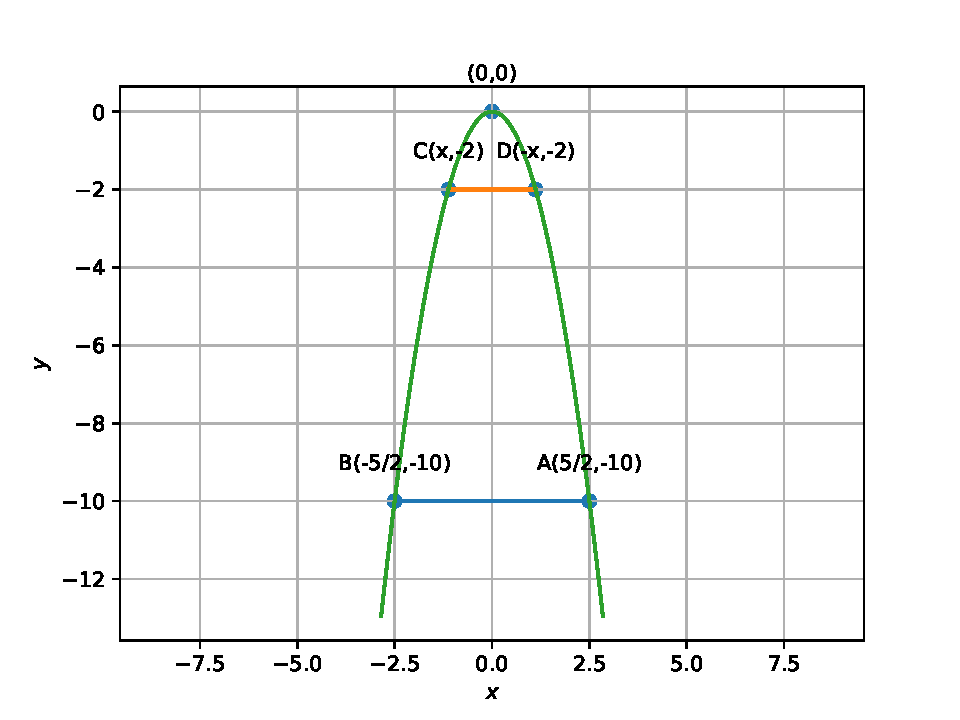
\includegraphics[width=\columnwidth]{chapters/11/11/5/2/figs/fig.pdf}
		\caption{}
		\label{fig:11/11/5/2}
  	\end{figure}
	\iffalse
} \vspace{5mm}

\section*{\large Solution}


Given, the axis of parabola is vertical,
\\ Let the equation of the axis be y-axis:
\begin{equation}
	\label{eq:parabola_q}
	\myvec{1\\0}\textbf{x}= 0
\end{equation}
\\ The above quadratic equation can be written in the general quadratic form as:

\begin{figure}[h]
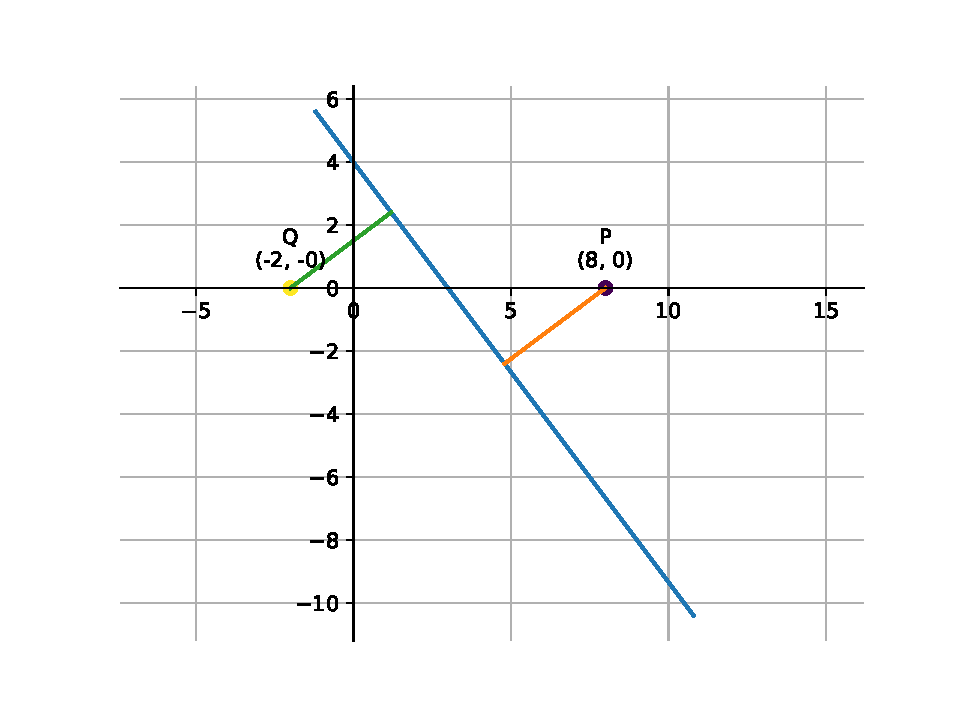
\includegraphics[width=0.8\columnwidth]{fig.pdf}
\end{figure}
\begin{equation}
	\label{eq:std_parabola}
	\textbf{x}^T\textbf{V}\textbf{x}+2\textbf{u}^T\textbf{x}+f=0
\end{equation}
where,
\begin{eqnarray}
\label{eq:Vec_V}
V = \myvec{1&0\\0&0}
\label{eq:Vec_U}
\\ u=\myvec{0\\2a}
\end{eqnarray}
\begin{equation}
\\ f =0
\end{equation}
Given arch is 10m high and 5m wide at the base. So the point $(\frac{5}{2},-10)$ lies on the parabola
\begin{equation}
	\myvec{X_1} = \myvec{\frac{5}{2}\\-10}
\end{equation}
\\ Substitute the point $X_1$ \\
\begin{eqnarray}
	\myvec{X_1}^T \myvec{V} \myvec{X_1} +2\myvec{u^T} \myvec{X_1} = 0
\\	a = \frac{5}{32}
\end{eqnarray}
\\Now , the matrix u will be,
\begin{equation}
	\myvec{u} = \myvec{0\\\frac{5}{16}}
\end{equation}
\\We need to find the width of parabola at a height of $2m$ from the vertex.So,the line parallel to x axis and passing through point $(0,-2)$ intersects the conic at 2 places C and D.
\\The line parallel to x-axis and passing through point $(0,-2)$ is
\begin{align}
	\myvec{X}\myvec{0\\1}^T = \myvec{2}
\end{align}
The points of intersection of the line 
\begin{align}
	L: \quad \vec{x} = \vec{q} + \mu \vec{m} \quad \mu \in \mathbf{R}
\label{eq:conic_tangent}
\end{align}
with the conic section  are given by
\begin{align}
\vec{x}_i = \vec{q} + \mu_i \vec{m}
\label{eq:conic_tangent_pts}
\end{align}
where 
{\tiny
\begin{multline}
\mu_i = \frac{1}
{
\vec{m}^T\vec{V}\vec{m}
}
\lbrak{-\vec{m}^T\brak{\vec{V}\vec{q}+\vec{u}}}
\\
\pm
\rbrak{\sqrt{
\sbrak{
\vec{m}^T\brak{\vec{V}\vec{q}+\vec{u}}
}^2
-
\brak
{
\vec{q}^T\vec{V}\vec{q} + 2\vec{u}^T\vec{q} +f
}
\brak{\vec{m}^T\vec{V}\vec{m}}
	}}
\label{eq:tangent_roots}
\end{multline}
}
\\
Substituting the line in the conic
\begin{align}
\brak{\vec{q} + \mu \vec{m}}^T\vec{V}\brak{\vec{q} + \mu \vec{m}}  
\\
+ 2 \vec{u}^T\brak{\vec{q} + \mu \vec{m}}+f &= 0
\\
\implies \mu^2\vec{m}^T\vec{V}\vec{m} + 2 \mu\vec{m}^T\brak{\vec{V}\vec{q}+\vec{u}} 
\\
+ \vec{q}^T\vec{V}\vec{q} + 2\vec{u}^T\vec{q} +f &= 0
\label{eq:conic_intercept}
\end{align}
Solving the above quadratic equations yeilds the roots.Let the point of intersections of line and curve be C and D.
\begin{align}
	C = q+ \mu_1m
	\\ D = q+ \mu_2m
\end{align}
\\The line CD will be
\begin{align}
	C-D = m(\mu_1-\mu_2)
	 \\ \textbf{m} = \myvec{1\\0}
\end{align}
The required width of parabola is the norm of the line CD.
\begin{align}
	||\boldsymbol{C-D}|| =
	2\sqrt{
\sbrak{
\vec{m}^T\brak{\vec{V}\vec{q}+\vec{u}}
}^2
-
\brak
{
\vec{q}^T\vec{V}\vec{q} + 2\vec{u}^T\vec{q} +f
}}
\end{align}
substitute the values of \vec{m},\vec{q},\vec{V} and \vec{u}
\begin{align}
	\frac{1}{2}||\vec{C-D}||^2 =
	\myvec{1&0}\brak{\vec{V}\myvec{0\\-2}+\vec{u}}\brak{\vec{V}\myvec{0\\-2}+\vec{u}}^T-
\end{align}
\begin{align*}
\brak
{
	\myvec{0&-2}\vec{V}\myvec{0\\-2} + 2\vec{u}^T\myvec{0\\-2} 
}
\end{align*}
 \begin{multiline}
	 \implies \sbrak{\myvec{1&0}\brak{\myvec{1&0\\0&0}\myvec{0\\-2} + \myvec{0\\\frac{5}{16}}}} \brak{\myvec{1&0\\0&0}\myvec{0\\-2} + \myvec{0\\\frac{5}{16}}}}^T  - \\
	 \\ \brak{\myvec{0&-2}\myvec{1&0\\0&0}\myvec{0\\-2} + 2\myvec{0 & \frac{5}{16}}\myvec{0\\-2} - 0} \\ \brak{\myvec{1&0}\myvec{1&0\\0&0}\myvec{1\\0}}
\end{multline}
\begin{align}
	\implies \sbrak{\myvec{1&0}\myvec{0\\\frac{5}{16}}}^2 - \brak{\myvec{0\\0}+2\myvec{0\\\frac{5}{-8}} - 0}(1) \\
 & = \myvec{5\\2}
\end{align}
\\The width of the Parabola at $2m$ height is the length of the line CD.  \begin{align} ||\vec{C-D}|| = \myvec{\sqrt{5}}$m$ \end{align} \section*{\large Construction} The input parameters are V,u,$X_1$,$y_2$ \\
\setlength\extrarowheight{7pt}
\begin{tabular}{|c|c|c|}
	\hline
	\textbf{Symbol}&\textbf{Value}&\textbf{Description}\\
	\hline
	$X_1$=\myvec{x_1\\y_1} & \myvec{\frac{5}{2}\\-10}&point at base \\[8pt]
	\hline
	$y_2$ & -2& height of point C\\[8pt]
	\hline
	$\vec{P}$&\myvec{0&1\\1&0}&eigenvectors of $\vec{V}$\\[8pt]
	\hline
	$\vec{c}$&$\myvec{0\\0}$&center of parabola\\
	\hline
	$\eta$&$\vec{u}^{\top}\vec{p}_1$&from Eq11\\[8pt]
	\hline
	$\lambda_2$&$\vec{e}_2^{\top}D\vec{e}_2$&from Eq9 \\[8pt]
	\hline
	$(\vec{A},\vec{B})$&\myvec{x_1&-x_1\\y_1&y_1}&points at the base\\[8pt]
	\hline
	$(\vec{C},\vec{D})$&\myvec{\sqrt{\frac{5y_2}{8}}&\sqrt{\frac{-5y_2}{8}}\\2&2}&points at 2m height\\[8pt]	\hline
\end{tabular}
\end{document}
\fi

\item  The cable of a uniformly loaded suspension bridge hangs in the form of a parabola. The roadway which is horizontal and 100 m long is supported by vertical wires attached to the cable, the longest wire being 30 m and the shortest being 6 m. Find the length of a supporting wire attached to the roadway 18 m from the middle.
\label{chapters/11/11/5/3}
\\
\solution
The parameters are then listed in  
    \tabref{tab:chapters/11/11/5/3/points}.
\begin{table}[H]
	\centering
    %%%%%%%%%%%%%%%%%%%%%%%%%%%%%%%%%%%%%%%%%%%%%%%%%%%%%%%%%%%%%%%%%%%%%%
%%                                                                  %%
%%  This is the header of a LaTeX2e file exported from Gnumeric.    %%
%%                                                                  %%
%%  This file can be compiled as it stands or included in another   %%
%%  LaTeX document. The table is based on the longtable package so  %%
%%  the longtable options (headers, footers...) can be set in the   %%
%%  preamble section below (see PRAMBLE).                           %%
%%                                                                  %%
%%  To include the file in another, the following two lines must be %%
%%  in the including file:                                          %%
%%        \def\inputGnumericTable{}                                 %%
%%  at the beginning of the file and:                               %%
%%        \input{name-of-this-file.tex}                             %%
%%  where the table is to be placed. Note also that the including   %%
%%  file must use the following packages for the table to be        %%
%%  rendered correctly:                                             %%
%%    \usepackage[latin1]{inputenc}                                 %%
%%    \usepackage{color}                                            %%
%%    \usepackage{array}                                            %%
%%    \usepackage{longtable}                                        %%
%%    \usepackage{calc}                                             %%
%%    \usepackage{multirow}                                         %%
%%    \usepackage{hhline}                                           %%
%%    \usepackage{ifthen}                                           %%
%%  optionally (for landscape tables embedded in another document): %%
%%    \usepackage{lscape}                                           %%
%%                                                                  %%
%%%%%%%%%%%%%%%%%%%%%%%%%%%%%%%%%%%%%%%%%%%%%%%%%%%%%%%%%%%%%%%%%%%%%%



%%  This section checks if we are begin input into another file or  %%
%%  the file will be compiled alone. First use a macro taken from   %%
%%  the TeXbook ex 7.7 (suggestion of Han-Wen Nienhuys).            %%
\def\ifundefined#1{\expandafter\ifx\csname#1\endcsname\relax}


%%  Check for the \def token for inputed files. If it is not        %%
%%  defined, the file will be processed as a standalone and the     %%
%%  preamble will be used.                                          %%
\ifundefined{inputGnumericTable}

%%  We must be able to close or not the document at the end.        %%
	\def\gnumericTableEnd{\end{document}}


%%%%%%%%%%%%%%%%%%%%%%%%%%%%%%%%%%%%%%%%%%%%%%%%%%%%%%%%%%%%%%%%%%%%%%
%%                                                                  %%
%%  This is the PREAMBLE. Change these values to get the right      %%
%%  paper size and other niceties.                                  %%
%%                                                                  %%
%%%%%%%%%%%%%%%%%%%%%%%%%%%%%%%%%%%%%%%%%%%%%%%%%%%%%%%%%%%%%%%%%%%%%%

	\documentclass[12pt%
			  %,landscape%
                    ]{report}
       
\begin{document}


%%  End of the preamble for the standalone. The next section is for %%
%%  documents which are included into other LaTeX2e files.          %%
\else

%%  We are not a stand alone document. For a regular table, we will %%
%%  have no preamble and only define the closing to mean nothing.   %%
\def\gnumericTableEnd{}

%%  If we want landscape mode in an embedded document, comment out  %%
%%  the line above and uncomment the two below. The table will      %%
%%  begin on a new page and run in landscape mode.                  %%
%       \def\gnumericTableEnd{\end{landscape}}
%       \begin{landscape}


%%  End of the else clause for this file being \input.              %%
\fi

%%%%%%%%%%%%%%%%%%%%%%%%%%%%%%%%%%%%%%%%%%%%%%%%%%%%%%%%%%%%%%%%%%%%%%
%%                                                                  %%
%%  The rest is the gnumeric table, except for the closing          %%
%%  statement. Changes below will alter the table's appearance.     %%
%%                                                                  %%
%%%%%%%%%%%%%%%%%%%%%%%%%%%%%%%%%%%%%%%%%%%%%%%%%%%%%%%%%%%%%%%%%%%%%%

\providecommand{\gnumericmathit}[1]{#1}
%%  Uncomment the next line if you would like your numbers to be in %%
%%  italics if they are italizised in the gnumeric table.           %%
%\renewcommand{\gnumericmathit}[1]{\mathit{#1}}
\providecommand{\gnumericPB}[1]%
{\let\gnumericTemp=\\#1\let\\=\gnumericTemp\hspace{0pt}}
\ifundefined{gnumericTableWidthDefined}
\newlength{\gnumericTableWidth}
\newlength{\gnumericTableWidthComplete}
\newlength{\gnumericMultiRowLength}
\global\def\gnumericTableWidthDefined{}
\fi
%% The following setting protects this code from babel shorthands.  %%
\ifthenelse{\isundefined{\languageshorthands}}{}{\languageshorthands{english}}
%%  The default table format retains the relative column widths of  %%
%%  gnumeric. They can easily be changed to c, r or l. In that case %%
%%  you may want to comment out the next line and uncomment the one %%
%%  thereafter                                                      %%
\providecommand\gnumbox{\makebox[0pt]}
%%\providecommand\gnumbox[1][]{\makebox}

%% to adjust positions in multirow situations                       %%
\setlength{\bigstrutjot}{\jot}
\setlength{\extrarowheight}{\doublerulesep}

%%  The \setlongtables command keeps column widths the same across  %%
%%  pages. Simply comment out next line for varying column widths.  %%
\setlongtables

\setlength\gnumericTableWidth{%
       53pt+%
       171pt+%
       53pt+%
       0pt}
\def\gumericNumCols{3}
\setlength\gnumericTableWidthComplete{\gnumericTableWidth+%
       \tabcolsep*\gumericNumCols*2+\arrayrulewidth*\gumericNumCols}
\ifthenelse{\lengthtest{\gnumericTableWidthComplete > \linewidth}}%
{\def\gnumericScale{1*\ratio{\linewidth-%
                     \tabcolsep*\gumericNumCols*2-%
                     \arrayrulewidth*\gumericNumCols}%
              {\gnumericTableWidth}}}%
{\def\gnumericScale{1}}

%%%%%%%%%%%%%%%%%%%%%%%%%%%%%%%%%%%%%%%%%%%%%%%%%%%%%%%%%%%%%%%%%%%%%%
%%                                                                  %%
%% The following are the widths of the various columns. We are      %%
%% defining them here because then they are easier to change.       %%
%% Depending on the cell formats we may use them more than once.    %%
%%                                                                  %%
%%%%%%%%%%%%%%%%%%%%%%%%%%%%%%%%%%%%%%%%%%%%%%%%%%%%%%%%%%%%%%%%%%%%%%

\ifthenelse{\isundefined{\gnumericColA}}{\newlength{\gnumericColA}}{}\settowidth{\gnumericColA}{\begin{tabular}{@{}p{40pt*\gnumericScale}@{}}x\end{tabular}}
\ifthenelse{\isundefined{\gnumericColB}}{\newlength{\gnumericColB}}{}\settowidth{\gnumericColB}{\begin{tabular}{@{}p{171pt*\gnumericScale}@{}}x\end{tabular}}
\ifthenelse{\isundefined{\gnumericColC}}{\newlength{\gnumericColC}}{}\settowidth{\gnumericColC}{\begin{tabular}{@{}p{60pt*\gnumericScale}@{}}x\end{tabular}}

\begin{tabular}[c]{%
              b{\gnumericColA}%
              b{\gnumericColB}%
              b{\gnumericColC}%
       }

       %%%%%%%%%%%%%%%%%%%%%%%%%%%%%%%%%%%%%%%%%%%%%%%%%%%%%%%%%%%%%%%%%%%%%%
       %%  The longtable options. (Caption, headers... see Goosens, p.124) %%
       %	\caption{The Table Caption.}             \\	%
       % \hline	% Across the top of the table.
       %%  The rest of these options are table rows which are placed on    %%
       %%  the first, last or every page. Use \multicolumn if you want.    %%

       %%  Header for the first page.                                      %%
       %	\multicolumn{3}{c}{The First Header} \\ \hline 
       %	\multicolumn{1}{c}{colTag}	%Column 1
       %	&\multicolumn{1}{c}{colTag}	%Column 2
       %	&\multicolumn{1}{c}{colTag}	\\ \hline %Last column
       %	\endfirsthead

       %%  The running header definition.                                  %%
       %	\hline
       %	\multicolumn{3}{l}{\ldots\small\slshape continued} \\ \hline
       %	\multicolumn{1}{c}{colTag}	%Column 1
       %	&\multicolumn{1}{c}{colTag}	%Column 2
       %	&\multicolumn{1}{c}{colTag}	\\ \hline %Last column
       %	\endhead

       %%  The running footer definition.                                  %%
       %	\hline
       %	\multicolumn{3}{r}{\small\slshape continued\ldots} \\
       %	\endfoot

       %%  The ending footer definition.                                   %%
       %	\multicolumn{3}{c}{That's all folks} \\ \hline 
       %	\endlastfoot
       %%%%%%%%%%%%%%%%%%%%%%%%%%%%%%%%%%%%%%%%%%%%%%%%%%%%%%%%%%%%%%%%%%%%%%

       \hhline{|-|-|-}
       \multicolumn{1}{|p{\gnumericColA}|}%
	{\gnumericPB {\centering}$\vec{O}$}
        & \multicolumn{1}{p{\gnumericColB}|} %
       {\gnumericPB{\raggedright}\gnumbox[l]{Lowest point of cable}}
        & \multicolumn{1}{p{\gnumericColC}|} %
       {\gnumericPB{\raggedright}\gnumbox[l]{\myvec{0 \\ 0}}}
       \\
       \hhline{|-|-|-|}
       \multicolumn{1}{|p{\gnumericColA}|}%
       {\gnumericPB{\raggedright}\gnumbox[l]{$d$}}
        & \multicolumn{1}{p{\gnumericColB}|} %
       {\gnumericPB{\raggedright}\gnumbox[l]{Length of the cable}}
        & \multicolumn{1}{p{\gnumericColC}|} %
       {\gnumericPB{\raggedright}\gnumbox[l]{100 m}}
       \\
       \hhline{|-|-|-|}
       \multicolumn{1}{|p{\gnumericColA}|}%
       {\gnumericPB{\raggedright}\gnumbox[l]{$d_1$}}
        & \multicolumn{1}{p{\gnumericColB}|} %
       {\gnumericPB{\raggedright}\gnumbox[l]{Length of longest wire}}
        & \multicolumn{1}{p{\gnumericColC}|} %
       {\gnumericPB{\raggedright}\gnumbox[l]{30 m}}
       \\
       \hhline{|-|-|-|}
       \multicolumn{1}{|p{\gnumericColA}|}%
       {\gnumericPB{\raggedright}\gnumbox[l]{$d_2$}}
        & \multicolumn{1}{p{\gnumericColB}|} %
       {\gnumericPB{\raggedright}\gnumbox[l]{Length of shortest wire}}
        & \multicolumn{1}{p{\gnumericColC}|} %
       {\gnumericPB{\raggedright}\gnumbox[l]{6 m}}
       \\
       \hhline{|-|-|-|}
       \multicolumn{1}{|p{\gnumericColA}|}%
       {\gnumericPB{\raggedright}$\vec{A}$}
        & \multicolumn{1}{p{\gnumericColB}|} %
       {\gnumericPB{\raggedright}\gnumbox[l]{End point of cable}}
        & \multicolumn{1}{p{\gnumericColC}|} %
       {\gnumericPB{\raggedright}\gnumbox[l]{\myvec{\frac{d}{2}\\d_1-d_2}}}
       \\
       \hhline{|-|-|-|}
       \multicolumn{1}{|p{\gnumericColA}|}%
       {\gnumericPB{\raggedright}$\vec{B}$}
        & \multicolumn{1}{p{\gnumericColB}|} %
       {\gnumericPB{\raggedright}\gnumbox[l]{End point of cable}}
        & \multicolumn{1}{p{\gnumericColC}|} %
       {\gnumericPB{\raggedright}\gnumbox[l]{\myvec{-\frac{d}{2}\\d_1-d_2}}}
       \\
       \hhline{|-|-|-|}

\end{tabular}

\ifthenelse{\isundefined{\languageshorthands}}{}{\languageshorthands{\languagename}}
\gnumericTableEnd
    \caption{points}
    \label{tab:chapters/11/11/5/3/points}
\end{table}
For the conic,
\begin{align}
    \vec{V} = \myvec{1&0\\0&0}.
\end{align}
Points $\vec{O}, \vec{A}$, and $\vec{B}$ are on conic, so we have
\begin{align}
	\vec{O}^{\top}\vec{V}\vec{O} + 2\vec{u}^{\top}\vec{O} + f &= 0\\
	\vec{A}^{\top}\vec{V}\vec{A} + 2\vec{u}^{\top}\vec{A} + f &= 0\\
	\vec{B}^{\top}\vec{V}\vec{B} + 2\vec{u}^{\top}\vec{B} + f &= 0	 
\end{align}
which can be expressed as
\begin{align}
	2\vec{O}^{\top}\vec{u} + f &= - \vec{O}^{\top}\vec{V}\vec{O}\\
	2\vec{A}^{\top}\vec{u} + f &= - \vec{A}^{\top}\vec{V}\vec{A}\\
	2\vec{B}^{\top}\vec{u} + f &= - \vec{B}^{\top}\vec{V}\vec{B}	
\end{align}
leading to the matrix equation
\begin{align}
	\myvec{2\vec{O}^{\top} & 1\\ 2\vec{A}^{\top} & 1\\ 2\vec{B}^{\top} & 1}\myvec{\vec{u} \\ f} = -\myvec{\vec{O}^{\top}\vec{V}\vec{O}\\ \vec{A}^{\top}\vec{V}\vec{A}\\ \vec{B}^{\top}\vec{V}\vec{B}}
\end{align}
Substituting numerical values in the above equation,
\begin{align}
    \myvec{0&0&1\\ 100&48&1\\ -100&48&1}\myvec{\vec{u} \\ f} = -\myvec{0\\-2500\\-2500}\\
    \implies f = 0 \text{ and } \vec{u} = \myvec{0\\-\frac{625}{12}}
\end{align}
So, the equation of the parabola is
\begin{align}
    \label{eq:chapters/11/11/5/3/parab1}  \vec{x}^{\top}\myvec{1&0\\0&0}\vec{x} + 2\myvec{0&-\frac{625}{12}}\vec{x} = 0 
\end{align}
The desired point can be expressed as
\begin{align}
	\vec{D} = \myvec{18 \\ x_2}
\end{align}
Substituting this in the parabola equation,
\begin{align}
    18^2 - \frac{6}{625}\lambda_2 = 0
    \\
\implies \lambda_2 = \frac{1944}{625}
\end{align}
Thus, the length of a supporting wire attached to the roadway $18 m$ from the middle is 
\begin{align}
     \lambda_2 + d_2 = \frac{5694}{625} m   
\end{align}
See  
    \figref{fig:chapters/11/11/5/3/parabola}.
\begin{figure}[H]
    \centering
    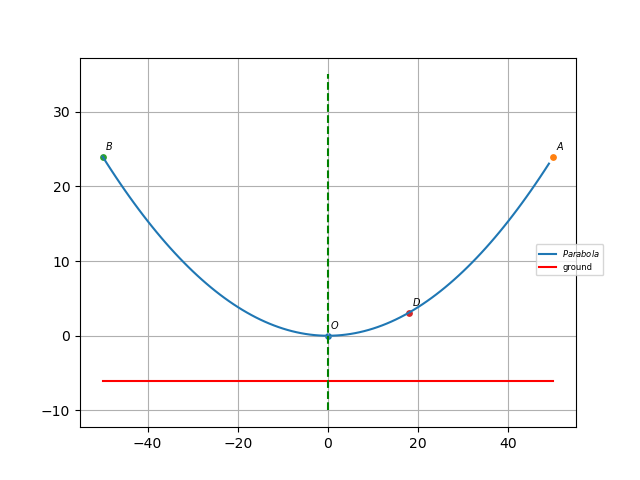
\includegraphics[width=0.75\columnwidth]{chapters/11/11/5/3/figs/parabola.png}
    \caption{}
    \label{fig:chapters/11/11/5/3/parabola}
\end{figure}


    \item Find the area of the triangle formed by the lines joining the vertex 
    of the parabola 
    \begin{align}
        x^2 = 12y
        \label{eq:chapters/11/11/5/6/parabola}
    \end{align}
    to the ends of its latus rectum.
\label{chapters/11/11/5/6}
		Rewriting \eqref{eq:chapters/11/11/5/6/parabola} in matrix form,
    \begin{align}
        \vec{x}^\top\myvec{1&0\\0&0}\vec{x} + 2\myvec{0&-6}\vec{x} = 0
        \label{eq:chapters/11/11/5/6/parabola-mtx}
    \end{align}
    The above parabola can be  expressed in standard form using 
\begin{align}
	\vec{x} = \vec{P}\vec{y} = \myvec{0 & 1 \\ 1 & 0}\vec{y}
        \label{eq:chapters/11/11/5/6/affine}
\end{align}
yielding
    \begin{align}
        \vec{y}^\top\myvec{0&0\\0&1}\vec{x} + 2\myvec{-6&0}\vec{x} = 0
        \label{eq:chapters/11/11/5/6/parabola-mty}
    \end{align}
    Hence, 
    from
\eqref{eq:conic_quad_form_nc}, 
    \begin{align}
	    \vec{n} = \vec{e}_1
        \label{eq:chapters/11/11/5/6/n}
	\\
	    c = -\frac{36}{2\times 6} = -3
    \end{align}
    Substituting in 
  \eqref{eq:conic_quad_form_F} 
  yields
    \begin{align}
        \vec{F} = 3\vec{e}_1
    \end{align}
    Thus, the equation of the latus rectum is
\begin{align}
        \vec{x} = \vec{F} + \kappa \vec{e}_2
        \label{eq:chapters/11/11/5/6/x-general}
    \end{align}
        Substituting in \eqref{eq:chapters/11/11/5/6/parabola-mty} and simplifying,
    \begin{align}
\kappa = \pm 6
        \label{eq:chapters/11/11/5/6/x-latus}
    \end{align}
    Thus, the ends of the latus rectum are
    \begin{align}
        \vec{y} = \myvec{3 \\ \pm 6}
    \end{align}
    The relevant parameters with respect to 
        \eqref{eq:chapters/11/11/5/6/parabola-mtx}
	can now be obtained using 
        \eqref{eq:chapters/11/11/5/6/affine}.
See \figref{fig:chapters/11/11/5/6/parabola}.
The area of the required triangle is
    \begin{align}
        \textrm{ar}\brak{\triangle OAB} = \frac{1}{2}\mydet{6&3\\-6&3} = 18 
    \end{align}
    \begin{figure}[H]
        \centering
        %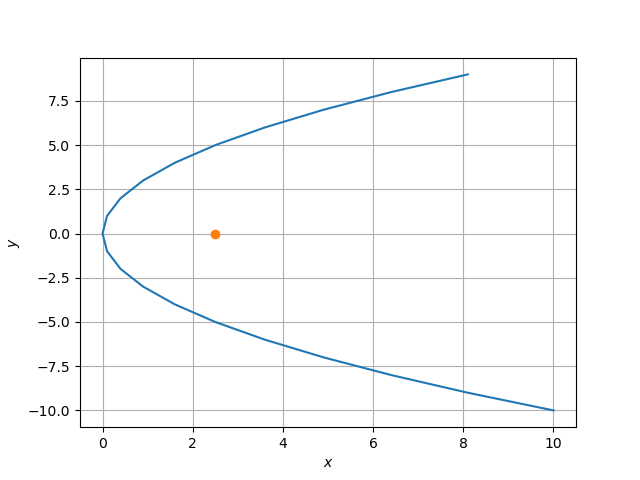
\includegraphics[width=0.75\columnwidth]{chapters/11/11/5/6/figs/parabola.png}
        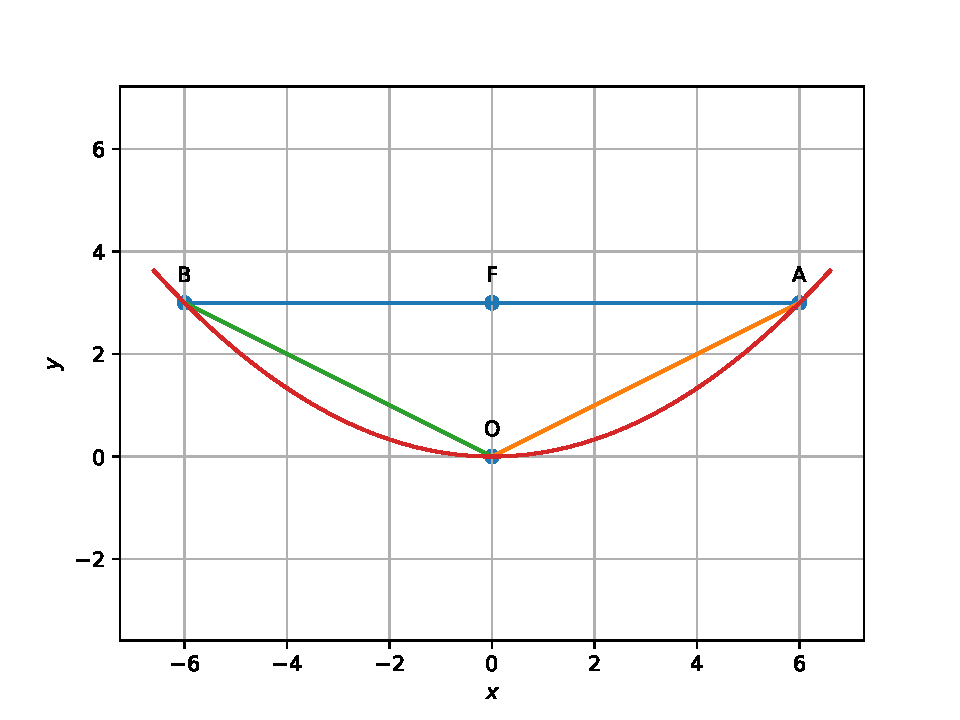
\includegraphics[width=0.75\columnwidth]{chapters/11/11/5/6/figs/fig1.pdf}
        \caption{}
        \label{fig:chapters/11/11/5/6/parabola}
    \end{figure}

\item An equilateral triangle is inscribed in the parabola $y^{2} = 4ax$,where one vertex is at the vertex of the parabola. Find the length of the side of the triangle.
\label{chapters/11/11/5/8}
\iffalse
\documentclass[journal,10pt,twocolumn]{article}
\usepackage{graphicx}
\usepackage[margin=0.5in]{geometry}
\usepackage[cmex10]{amsmath}
\usepackage{array}
\usepackage{booktabs}
\usepackage{mathtools}
\usepackage{amssymb}
\title{\textbf{Conics Assignment}}
\author{Alavala Chinnapa Reddy}
\date{September 2022}
\providecommand{\norm}[1]{\left\lVert#1\right\rVert}
\providecommand{\abs}[1]{\left\vert#1\right\vert}
\let\vec\mathbf
\newcommand{\myvec}[1]{\ensuremath{\begin{pmatrix}#1\end{pmatrix}}}
\newcommand{\mydet}[1]{\ensuremath{\begin{vmatrix}#1\end{vmatrix}}}
\providecommand{\brak}[1]{\ensuremath{\left(#1\right)}}
\providecommand{\lbrak}[1]{\ensuremath{\left(#1\right.}}
\providecommand{\rbrak}[1]{\ensuremath{\left.#1\right)}}
\providecommand{\sbrak}[1]{\ensuremath{{}\left[#1\right]}}
\begin{document}

\maketitle
\paragraph{\textit{Problem Statement} -
\fi
An equilateral triangle is inscribed in the parabola $y^{2} = 4ax$,where one vertex is at the vertex of the parabola. Find the length of the side of the triangle.
	\begin{figure}[!ht]
		\centering
 \includegraphics[width=\columnwidth]{chapters/11/11/5/8/figs/co.pdf}
		\caption{}
		\label{fig:11/11/5/8}
  	\end{figure}
\\
\solution
\iffalse
} \vspace{5mm}
\section*{\large Solution}


Given, the axis of parabola is horizotal.
\\ Given,one vertex of $\triangle$OAB is at vertex of parabola.

\begin{figure}[h]
\includegraphics[width=0.8\columnwidth]{figs/co.pdf}
\end{figure}
\begin{equation}
  \label{eq:std_parabola}
  \textbf{x}^T\textbf{V}\textbf{x}+2\textbf{u}^T\textbf{x}+f=0
\end{equation}
where,
\begin{eqnarray}
	\vec{O}=\myvec{0\\0}
\end{eqnarray}	
Equation Parabola is $y^2=4ax$\\
From $\triangle$OAB
\begin{eqnarray}
	\norm{\vec{A}}=\norm{\vec{B}}=\norm{\vec{A-B}}\\
	\norm{\vec{A}}^2=\norm{\vec{B}}^2=\norm{\vec{A-B}}^2\\
	\norm{\vec{A}}^2+\norm{\vec{B}}^2-2\vec{A}^T\vec{B}=\norm{\vec{A}}^2=\norm{\vec{B}}^2\\
	\frac{\vec{A}^T\vec{B}}{\norm{\vec{A}}^2}=\frac{\vec{A}^T\vec{B}}{\norm{\vec{B}^2}}=\frac{1}{2}
\end{eqnarray}
$\triangle$OAB is a equilateral triangle\\
$\alpha$=$60^{0}$\\
The side length of equilateral triangle,OA=OB=AB=r\\
Let
\begin{eqnarray}
	\vec{A}=\myvec{r\cos{\theta_1}\\r\sin{\theta_1}}\\
	\vec{B}=\myvec{r\cos{\theta_2}\\r\sin{\theta_2}}
\end{eqnarray}
\begin{eqnarray}
	\vec{A}^T\vec{B}=\frac{\norm{\vec{A}}^2}{2}\\
	r^2\cos{(\theta_1-\theta_2)}=\frac{r^2}{2}\\
	\theta_1-\theta_2=\cos{^{-1}\frac{1}{2}}
\end{eqnarray}
Given $\vec{A}$ satisfy the eq1
\begin{eqnarray}
	\vec{A}^T\vec{V}\vec{A}+2\vec{u}^T\vec{A}+f=0\\
	\vec{A}^T\vec{V}\vec{A}+2\vec{u}^T\vec{A}=0
\end{eqnarray}
\begin{equation}
	\myvec{r\cos{\theta_1}&r\sin{\theta_1}}\myvec{0&0\\0&1}\myvec{r\cos{\theta_1}\\r\sin{\theta_1}}+2\myvec{-2a&0}\myvec{r\cos{\theta_1}\\r\sin{\theta_1}}=0
\end{equation}
\begin{equation}
	\myvec{r\cos{\theta_1}&r\sin{\theta_1}}\myvec{0\\r\sin{\theta_1}}+2(-2ar\cos{\theta_1})=0
\end{equation}
\begin{eqnarray}
	r^2\sin{^2\theta_1}=4ar\cos{\theta_1}\\
	r=\frac{4a\cos{\theta_1}}{\sin{^2\theta_1}}
\end{eqnarray}
Similarly $\vec{B}$ satisfy the eq1
\begin{equation}
	r=\frac{4a\cos{\theta_2}}{\sin{^2\theta_2}}
\end{equation}
Form eq17 and eq18\\
Yeilding
\begin{eqnarray}
	\cos{(\theta_1+\theta_2)}=1\\
	\theta_1+\theta_2=\cos{^{-1}1}
\end{eqnarray}
Add eq11 and eq20\\
\begin{equation}
	\theta_1=\frac{\cos{^{-1}\frac{1}{2}+\cos{^{-1}1}}}{2}
\end{equation}
Subtract eq20 from eq11
\begin{equation}   
\theta_2=\frac{-\cos{^{-1}\frac{1}{2}+\cos{^{-1}1}}}{2}        
\end{equation}
 \section*{\large Construction} The input parameters are V,u,f \\
 $\vec{V}=\myvec{0&0\\0&1},\vec{u}=\myvec{-2a\\0},f=0$\\
\setlength\extrarowheight{7pt}
\begin{tabular}{|c|c|c|}
  \hline
  \textbf{Symbol}&\textbf{Value}&\textbf{Description}\\
  \hline
	a&1&\\
  \hline
	$\alpha$&$60^{0}$&$\angle{A}=\angle{B}=\angle{O}$\\
	\hline
	r&Solving eq18&OA=OB=AB\\
	\hline
  $\vec{O}$&$\myvec{0\\0}$&center of parabola and Point O\\
  \hline
	$\vec{A}$&$\myvec{r\cos{\theta_1}\\r\sin{\theta_1}}$&Point A\\[8pt]
  \hline
	$\vec{B}$&$\myvec{r\cos{\theta_2}\\r\sin{\theta_2}}$&Point B\\[8pt]  \hline
\end{tabular}
\end{document}
\fi

\end{enumerate}
In the each of the following Exercises, find the coordinates of the focus, axis of the parabola, the equation of the directrix and the length of the latus rectum.
\begin{enumerate}[label=\thesection.\arabic*,ref=\thesection.\theenumi,resume*]
\numberwithin{equation}{enumi}
\numberwithin{figure}{enumi}
\numberwithin{table}{enumi}

\item $y^2$=12x 
\label{chapters/11/11/2/1}
\\
\solution
See 
\tabref{tab:std-conic-params-sol}
and 
\figref{fig:11/11/2/1Fig1}.
\begin{figure}[!h]
	\begin{center}
		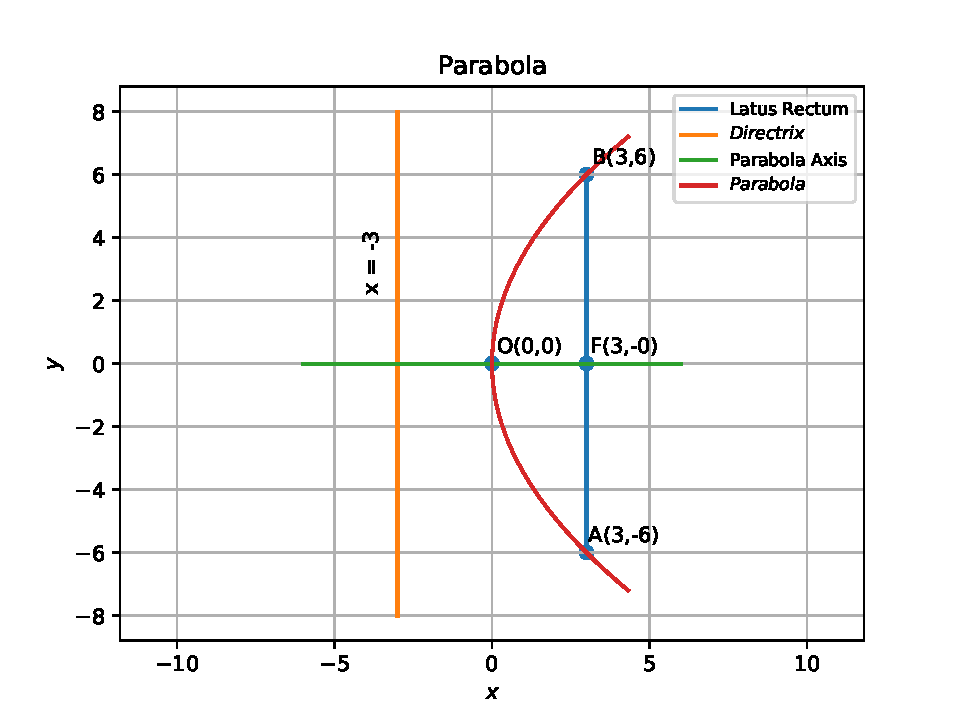
\includegraphics[width=\columnwidth]{chapters/11/11/2/1/figs/problem1.pdf}
	\end{center}
\caption{}
\label{fig:11/11/2/1Fig1}
\end{figure}



\item $x^2$=6y 
\\
\solution
\iffalse
\documentclass[12pt]{article}
\usepackage{graphicx}
\usepackage{amsmath}
\usepackage{mathtools}
\usepackage{gensymb}

\newcommand{\mydet}[1]{\ensuremath{\begin{vmatrix}#1\end{vmatrix}}}
\providecommand{\brak}[1]{\ensuremath{\left(#1\right)}}
\providecommand{\norm}[1]{\left\lVert#1\right\rVert}
\newcommand{\solution}{\noindent \textbf{Solution: }}
\newcommand{\myvec}[1]{\ensuremath{\begin{pmatrix}#1\end{pmatrix}}}
\let\vec\mathbf

\begin{document}
\begin{center}
\textbf\large{CONIC SECTIONS}

\end{center}
\section*{Excercise 11.2}

Q2.Find the coordinates of the focus, axis of the parabola, the equation of the directrix and the length of the latus rectum of a parabola whose equation is given by $x^2=6y$.

\solution
\fi
The given equation of the parabola can be rearranged as
\begin{align}
	\label{eq:chapters/11/11/2/2/parabolaEq1}
	x^2-6y=0
\end{align}
The above equation can be equated to the generic equation of conic sections
\begin{align}
	\label{eq:chapters/11/11/2/2/parabolaEq2}
	g\brak{\vec{x}}=\vec{x}^\top \vec{V}\vec{x}+2\vec{u}^\top \vec{x}+f=0
\end{align}
Comparing the coefficients of both equations \eqref{eq:chapters/11/11/2/2/parabolaEq1} and \eqref{eq:chapters/11/11/2/2/parabolaEq2}
\begin{align}
	\label{eq:chapters/11/11/2/2/eqV}
	\vec{V} &= \myvec{1&0\\0&0}\\
	\label{eq:chapters/11/11/2/2/eqU}
	\vec{u} &= -\myvec{0\\3}\\
	\label{eq:chapters/11/11/2/2/eqF}
	f &= 0
\end{align}
\begin{enumerate}
\item From equation \eqref{eq:chapters/11/11/2/2/eqV}, since $\vec{V}$ is already diagonalized, the Eigen values $\lambda_1 \text{ and } \lambda_2$ are given as
\begin{align}
	\label{eq:chapters/11/11/2/2/eqEigen1}
	\lambda_1 &= 1\\
	\label{eq:chapters/11/11/2/2/eqEigen2}
	\lambda_2 &= 0
\end{align}
And the corresponding eigen vector matrix $\vec{P}$ is indentity, so the Eigen vector $\vec{p}_2$ corresponding to Eigen value $\lambda_2$ is
\begin{align}
	\vec{p}_2 &= \myvec{0\\1}\\
	\vec{n} &= \sqrt{\lambda_1}\vec{p}_2\\
		&= \sqrt{1}\myvec{0\\1}\\
		&= \myvec{0\\1}
\end{align}
Now,
\begin{align}
	\label{eq:chapters/11/11/2/2/eqC}
	c = \frac{\norm{\vec{u}}^2 - \lambda_1 f}{2\vec{u}^\top \vec{n}}
\end{align}
Substituting values of $\vec{u},\vec{n},\lambda_1 \text{ and } f$ in \eqref{eq:chapters/11/11/2/2/eqC}
\begin{align}
	c = \frac{3^2-1\brak{0}}{-2\myvec{0&3}\myvec{0\\1}} = -\frac{3}{2}
\end{align}
The focus $\vec{F}$ of parabola is expressed as
\begin{align}
	\vec{F} &= \frac{ce^2 \vec{n}-\vec{u}}{\lambda_1}\\
		&= \frac{-\frac{3}{2}\brak{1}^2 \myvec{0\\1}+\myvec{0\\3}}{1}\\
		&= \myvec{0\\\frac{3}{2}}
\end{align}
\item Equation of directrix is given as
\begin{align}
	\vec{n}^\top \vec{x} &= c\\
	\myvec{0&1}\vec{x} &= -\frac{3}{2}
\end{align}
\item The equation for the axis of parabola passing through $\vec{F}$ and orthogonal to the directrix is given as
\begin{align}
	\label{eq:chapters/11/11/2/2/eqM}
	\vec{m}^\top \brak{\vec{x}-\vec{F}} = 0
\end{align}
where $\vec{m}$ is the normal vector to the axis and also the slope of the directrix. Now since
\begin{align}
	\vec{n} = \myvec{0\\1}\\
	\vec{m} = \myvec{1\\0}
\end{align}
Substituting in \eqref{eq:chapters/11/11/2/2/eqM}
\begin{align}
	\myvec{1&0}\myvec{\vec{x}-\myvec{0\\\frac{3}{2}}}&=0\\
	\myvec{1&0}\vec{x} &= 0
\end{align}
\item The latus rectum of a parabola is given by
\begin{align}
	l&=\frac{\eta}{\lambda_1}\\
	 &=\frac{2\vec{u}^\top \vec{p}_2}{\lambda_1}\\
	 &=\frac{2\myvec{0&3}\myvec{0\\1}}{1}\\
	 &=6 \text{ units }
\end{align}
See Fig. \ref{fig:chapters/11/11/2/2/Fig1}
\begin{figure}[!h]
	\begin{center} 
	    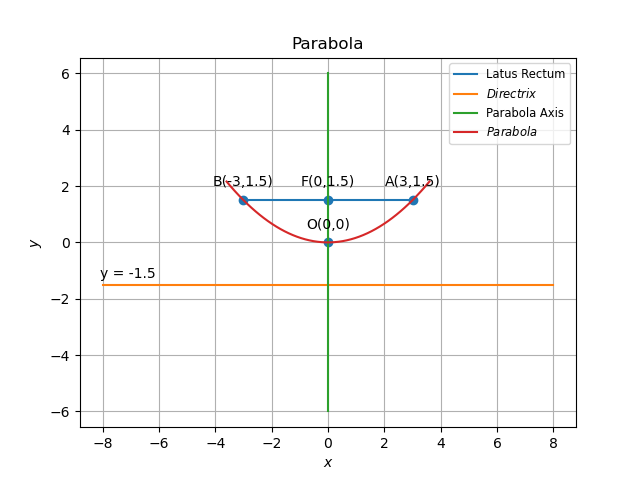
\includegraphics[width=\columnwidth]{chapters/11/11/2/2/figs/parabola}
	\end{center}
\caption{}
\label{fig:chapters/11/11/2/2/Fig1}
\end{figure}
\end{enumerate}





\item Find the coordinates of the focus, axis of the
parabola, the equation of the directrix and the length of the latus rectum of $y^2 = –8x$
\\
\solution
See \tabref{tab:std-conic-params-sol} and 
\figref{fig:chapters/11/11/2/3/1}.
\begin{figure}[H]
\centering
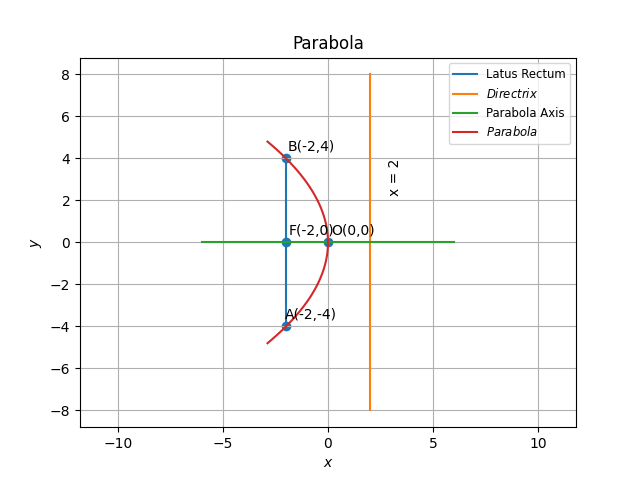
\includegraphics[width=0.75\columnwidth]{chapters/11/11/2/3/figs/fig.png}
\caption{Graph}
\label{fig:chapters/11/11/2/3/1}
\end{figure}

\item $y^2$=-8x

\item $x^2$=-16y
\\
\solution
See \tabref{tab:rot-conic-params-sol}
and 
\figref{fig:chapters/11/11/2/4/Fig1}.
\begin{figure}[!h]
	\begin{center} 
	    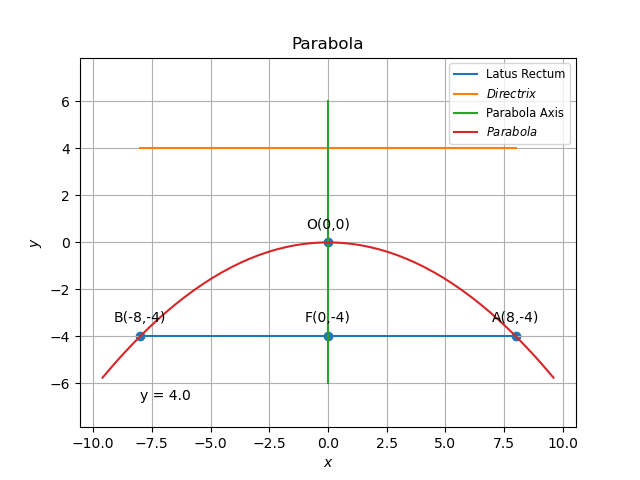
\includegraphics[width=\columnwidth]{chapters/11/11/2/4/figs/parabola}
	\end{center}
\caption{}
\label{fig:chapters/11/11/2/4/Fig1}
\end{figure}


\item $y^2$=10x  

\item $x^2$=-9y  
\end{enumerate}

Each of the Exercises, find the equation of the parabola, that satisfies the given conditions.

\begin{enumerate}[label=\thesection.\arabic*,ref=\thesection.\theenumi,resume*]
\item Focus(6,0); directrix x=-6 
\item Focus(0,-3); directrix y=3
\item Vertex(0,0); Focus(3,0)
\item Vertex(0,0); Focus(-2,0) 
\item Vertex(0,0) passing through(2,3) and axis is along x-axis
\item Vertex(0,0) passing through(5,2) symmetric with respect to y-axis
\end{enumerate}
